% Learning flowcharts for usgs-splib07.
%   Page 1: the whole pipeline, from download to features.
%   Page 2: what happens to ONE spectrum, step by step.
% Build:  pdflatex workflow.tex      (needs TikZ only)
\documentclass[tikz,border=10pt,multi=tikzpicture]{standalone}
\usepackage[T1]{fontenc}
\usepackage{lmodern}
\hyphenpenalty=10000 \exhyphenpenalty=10000
\usetikzlibrary{arrows.meta,positioning,fit,backgrounds,shapes.geometric,calc}

\newcommand{\fn}[1]{{\ttfamily\scriptsize\color{black!75}#1}}
\definecolor{cDown}{HTML}{2F6DB5}
\definecolor{cCat}{HTML}{2E8B57}
\definecolor{cBuild}{HTML}{B8860B}
\definecolor{cPre}{HTML}{8E44AD}
\definecolor{cFeat}{HTML}{C0392B}

\tikzset{
  box/.style={rectangle, rounded corners=3pt, draw=#1!70!black, fill=#1!12, thick,
    minimum width=4.7cm, minimum height=1.9cm, text width=4.4cm, align=center,
    font=\footnotesize, inner sep=3pt},
  fn/.style={font=\ttfamily\scriptsize, text=black!75},
  arr/.style={-{Stealth[length=2.8mm]}, thick, draw=black!70},
  dec/.style={diamond, aspect=2.3, draw=orange!70!black, fill=orange!15, thick,
    text width=2.3cm, align=center, font=\scriptsize, inner sep=0pt},
  small/.style={rectangle, rounded corners=3pt, draw=black!50, fill=black!5, thick,
    text width=3cm, align=center, font=\scriptsize, inner sep=3pt},
  phase/.style={rounded corners=7pt, draw=#1!55, fill=#1!5, inner sep=9pt, thick, dashed},
  plab/.style={font=\bfseries\small, text=#1!60!black, anchor=south west},
  note/.style={font=\scriptsize\itshape, text=black!65, align=left},
}

\begin{document}

% ============================================================ PAGE 1
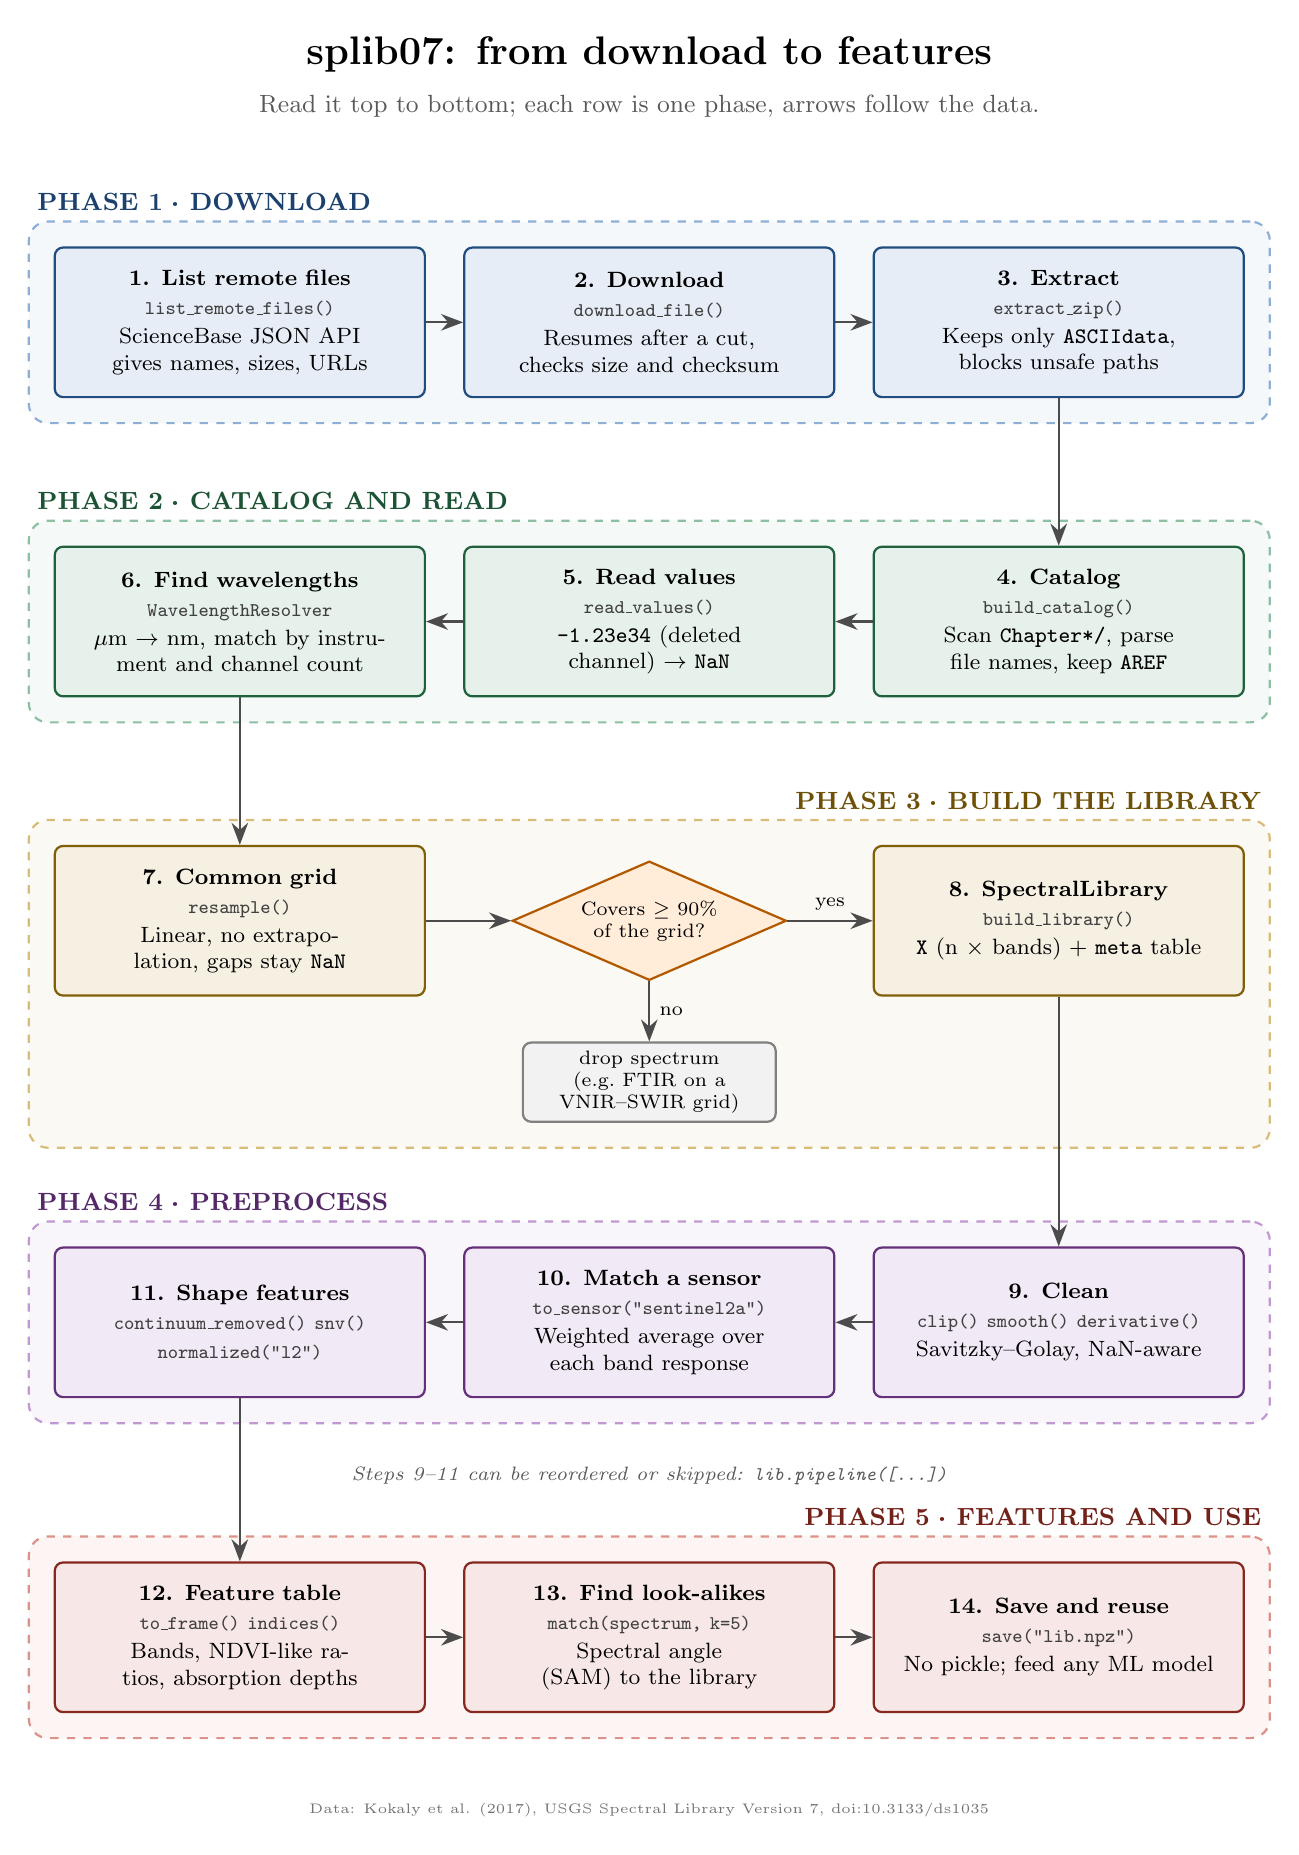
\begin{tikzpicture}
  \node[font=\Large\bfseries] at (5.2,3.4) {splib07: from download to features};
  \node[font=\small, text=black!65] at (5.2,2.75)
    {Read it top to bottom; each row is one phase, arrows follow the data.};

  % ---- Phase 1: download (left to right)
  \node[box=cDown] (n1) at (0,0)    {\textbf{1. List remote files}\\[1pt]\fn{list\_remote\_files()}\\[1pt]ScienceBase JSON API gives names, sizes, URLs};
  \node[box=cDown] (n2) at (5.2,0)  {\textbf{2. Download}\\[1pt]\fn{download\_file()}\\[1pt]Resumes after a cut, checks size and checksum};
  \node[box=cDown] (n3) at (10.4,0) {\textbf{3. Extract}\\[1pt]\fn{extract\_zip()}\\[1pt]Keeps only \texttt{ASCIIdata}, blocks unsafe paths};
  \draw[arr] (n1) -- (n2); \draw[arr] (n2) -- (n3);

  % ---- Phase 2: catalog and read (right to left)
  \node[box=cCat] (n4) at (10.4,-3.8) {\textbf{4. Catalog}\\[1pt]\fn{build\_catalog()}\\[1pt]Scan \texttt{Chapter*/}, parse file names, keep \texttt{AREF}};
  \node[box=cCat] (n5) at (5.2,-3.8)  {\textbf{5. Read values}\\[1pt]\fn{read\_values()}\\[1pt]\texttt{-1.23e34} (deleted channel) $\to$ \texttt{NaN}};
  \node[box=cCat] (n6) at (0,-3.8)    {\textbf{6. Find wavelengths}\\[1pt]\fn{WavelengthResolver}\\[1pt]$\mu$m $\to$ nm, match by instrument and channel count};
  \draw[arr] (n3) -- (n4); \draw[arr] (n4) -- (n5); \draw[arr] (n5) -- (n6);

  % ---- Phase 3: build (left to right)
  \node[box=cBuild] (n7) at (0,-7.6)   {\textbf{7. Common grid}\\[1pt]\fn{resample()}\\[1pt]Linear, no extrapolation, gaps stay \texttt{NaN}};
  \node[dec]        (n8) at (5.2,-7.6) {Covers $\ge$ 90\% of the grid?};
  \node[box=cBuild] (n9) at (10.4,-7.6){\textbf{8. SpectralLibrary}\\[1pt]\fn{build\_library()}\\[1pt]\texttt{X} (n $\times$ bands) + \texttt{meta} table};
  \node[small] (drop) at (5.2,-9.65) {drop spectrum (e.g.\ FTIR on a VNIR--SWIR grid)};
  \draw[arr] (n6) -- (n7); \draw[arr] (n7) -- (n8);
  \draw[arr] (n8) -- node[above,font=\scriptsize]{yes} (n9);
  \draw[arr] (n8) -- node[right,font=\scriptsize]{no} (drop);

  % ---- Phase 4: preprocess (right to left)
  \node[box=cPre] (n10) at (10.4,-12.7) {\textbf{9. Clean}\\[1pt]\fn{clip()  smooth()  derivative()}\\[1pt]Savitzky--Golay, NaN-aware};
  \node[box=cPre] (n11) at (5.2,-12.7)  {\textbf{10. Match a sensor}\\[1pt]\fn{to\_sensor("sentinel2a")}\\[1pt]Weighted average over each band response};
  \node[box=cPre] (n12) at (0,-12.7)    {\textbf{11. Shape features}\\[1pt]\fn{continuum\_removed()  snv()}\\[1pt]\fn{normalized("l2")}};
  \draw[arr] (n9) -- (n10); \draw[arr] (n10) -- (n11); \draw[arr] (n11) -- (n12);
  \node[note] at (5.2,-14.65) {Steps 9--11 can be reordered or skipped: \texttt{lib.pipeline([...])}};

  % ---- Phase 5: features and use (left to right)
  \node[box=cFeat] (n13) at (0,-16.7)    {\textbf{12. Feature table}\\[1pt]\fn{to\_frame()  indices()}\\[1pt]Bands, NDVI-like ratios, absorption depths};
  \node[box=cFeat] (n14) at (5.2,-16.7)  {\textbf{13. Find look-alikes}\\[1pt]\fn{match(spectrum, k=5)}\\[1pt]Spectral angle (SAM) to the library};
  \node[box=cFeat] (n15) at (10.4,-16.7) {\textbf{14. Save and reuse}\\[1pt]\fn{save("lib.npz")}\\[1pt]No pickle; feed any ML model};
  \draw[arr] (n12) -- (n13); \draw[arr] (n13) -- (n14); \draw[arr] (n14) -- (n15);

  % ---- phase backgrounds
  \begin{scope}[on background layer]
    \node[phase=cDown,  fit=(n1)(n2)(n3), label={[plab=cDown]north west:PHASE 1 \textperiodcentered\ DOWNLOAD}] {};
    \node[phase=cCat,   fit=(n4)(n5)(n6), label={[plab=cCat]north west:PHASE 2 \textperiodcentered\ CATALOG AND READ}] {};
    \node[phase=cBuild, fit=(n7)(n8)(n9)(drop), label={[plab=cBuild, anchor=south east]north east:PHASE 3 \textperiodcentered\ BUILD THE LIBRARY}] {};
    \node[phase=cPre,   fit=(n10)(n11)(n12), label={[plab=cPre]north west:PHASE 4 \textperiodcentered\ PREPROCESS}] {};
    \node[phase=cFeat,  fit=(n13)(n14)(n15), label={[plab=cFeat, anchor=south east]north east:PHASE 5 \textperiodcentered\ FEATURES AND USE}] {};
  \end{scope}

  \node[font=\tiny, text=black!55] at (5.2,-18.9)
    {Data: Kokaly et al. (2017), USGS Spectral Library Version 7, doi:10.3133/ds1035};
\end{tikzpicture}

% ============================================================ PAGE 2
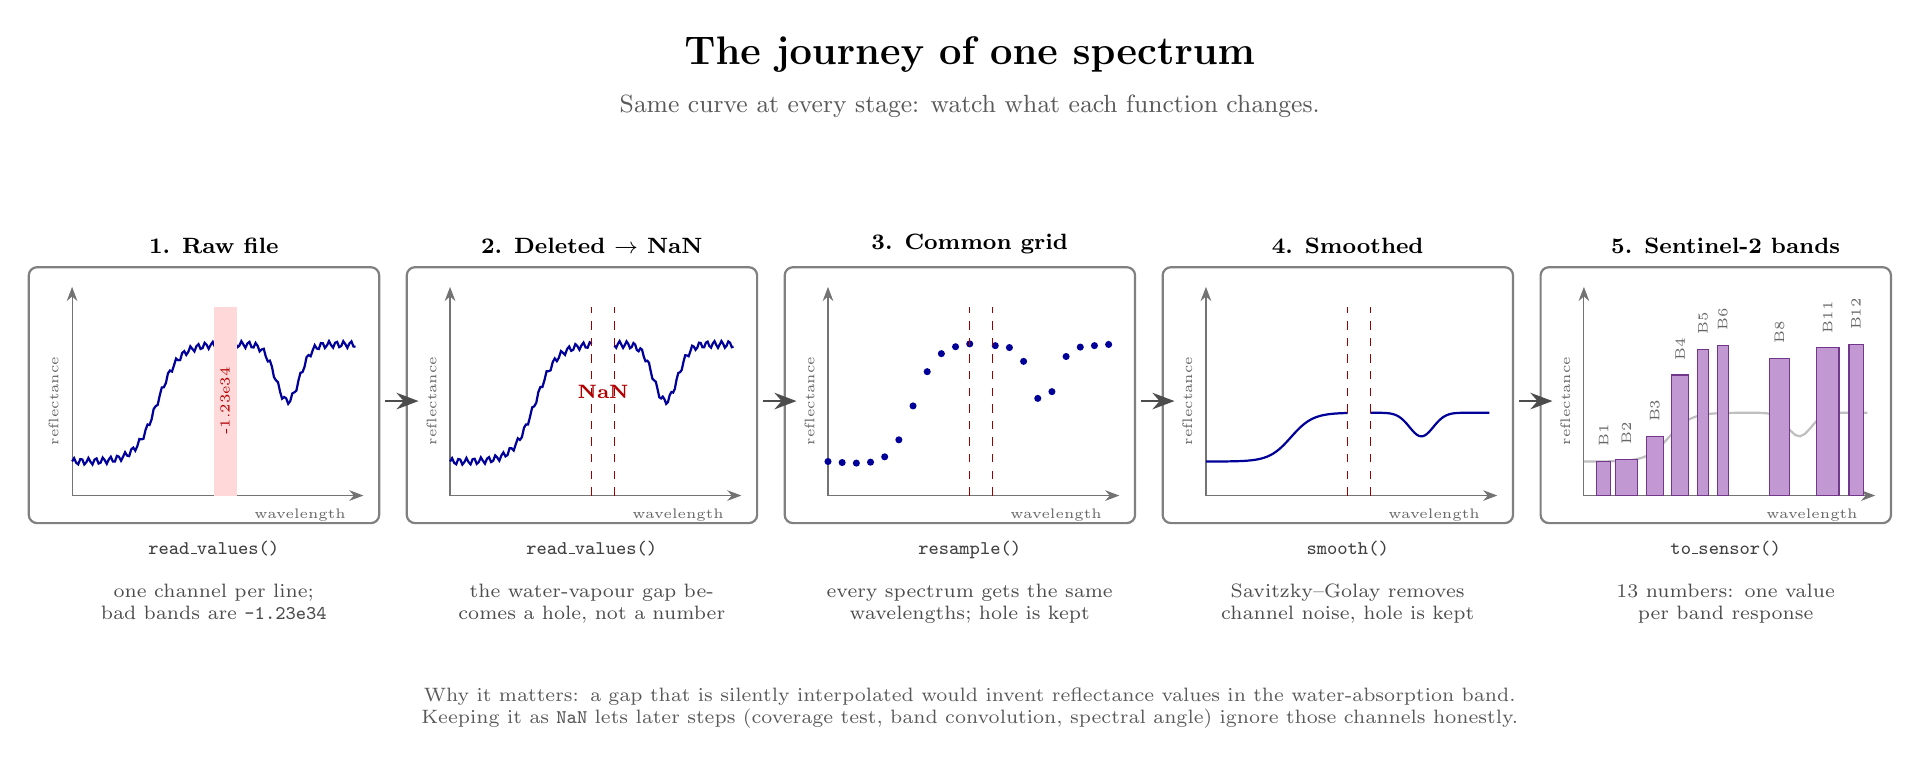
\begin{tikzpicture}[x=1cm,y=1cm]
  \node[font=\Large\bfseries] at (11.4,5.6) {The journey of one spectrum};
  \node[font=\small, text=black!65] at (11.4,4.95) {Same curve at every stage: watch what each function changes.};

  % curve: absorption dip near x=7.5, red-edge-like rise near x=3
  \def\spec#1{0.18+0.62/(1+exp(max(-8,min(8,-(#1-3)*2.6))))-0.30*exp(max(-8,-((#1-7.6)^2)/0.35))}
  \def\w{3.6}   % panel width (cm), x runs 0..10 -> scaled
  \def\h{2.4}   % panel height (cm)
  \pgfmathsetmacro{\sx}{\w/10}

  \foreach \i/\title/\code/\caption in {
    0/{1. Raw file}/{read\_values()}/{one channel per line; bad bands are \texttt{-1.23e34}},
    1/{2. Deleted $\to$ NaN}/{read\_values()}/{the water-vapour gap becomes a hole, not a number},
    2/{3. Common grid}/{resample()}/{every spectrum gets the same wavelengths; hole is kept},
    3/{4. Smoothed}/{smooth()}/{Savitzky--Golay removes channel noise, hole is kept},
    4/{5. Sentinel-2 bands}/{to\_sensor()}/{13 numbers: one value per band response}} {
    \pgfmathsetmacro{\ox}{\i*4.8}
    \begin{scope}[shift={(\ox,0)}]
      \draw[rounded corners=3pt, draw=black!50, fill=white, thick] (-0.55,-0.35) rectangle (\w+0.3,\h+0.5);
      \draw[black!55, -{Stealth[length=1.8mm]}] (0,0) -- (\w+0.1,0);
      \node[font=\tiny, anchor=north east, text=black!60] at (\w,-0.04) {wavelength};
      \draw[black!55, -{Stealth[length=1.8mm]}] (0,0) -- (0,\h+0.25);
      \node[font=\tiny, rotate=90, anchor=south, text=black!60] at (-0.05,\h/2) {reflectance};
      \node[font=\footnotesize\bfseries, anchor=south] at (\w/2,\h+0.55) {\title};
      \node[fn, anchor=north, text width=3.9cm, align=center] at (\w/2,-0.45) {\code};
      \node[font=\scriptsize, text width=3.9cm, align=center, anchor=north, text=black!70] at (\w/2,-1.0) {\caption};
    \end{scope}
  }

  % panel 0: raw jagged curve, bad band drawn as a red spike line
  \begin{scope}[shift={(0,0)}]
    \draw[blue!60!black, thick, samples=140, domain=0:10, variable=\t]
      plot ({\sx*\t}, {\h*(\spec{\t}+0.018*sin(mod(\t*1400,360)))});
    \fill[red!15] ({\sx*5.0},0) rectangle ({\sx*5.8},\h);
    \node[font=\tiny, text=red!70!black, rotate=90] at ({\sx*5.4},{\h*0.5}) {-1.23e34};
  \end{scope}

  % panel 1: same, with a visible hole
  \begin{scope}[shift={(4.8,0)}]
    \draw[blue!60!black, thick, samples=70, domain=0:5.0, variable=\t]
      plot ({\sx*\t}, {\h*(\spec{\t}+0.018*sin(mod(\t*1400,360)))});
    \draw[blue!60!black, thick, samples=70, domain=5.8:10, variable=\t]
      plot ({\sx*\t}, {\h*(\spec{\t}+0.018*sin(mod(\t*1400,360)))});
    \node[font=\scriptsize\bfseries, text=red!70!black] at ({\sx*5.4},{\h*0.55}) {NaN};
    \draw[red!60!black, dashed] ({\sx*5.0},0) -- ({\sx*5.0},\h) ({\sx*5.8},0) -- ({\sx*5.8},\h);
  \end{scope}

  % panel 2: grid points (dots) with hole
  \begin{scope}[shift={(9.6,0)}]
    \foreach \t in {0,0.5,...,5.0,5.9,6.4,...,10} {
      \fill[blue!60!black] ({\sx*\t},{\h*(\spec{\t}+0.018*sin(mod(\t*1400,360)))}) circle (0.045);
    }
    \draw[red!60!black, dashed] ({\sx*5.0},0) -- ({\sx*5.0},\h) ({\sx*5.8},0) -- ({\sx*5.8},\h);
  \end{scope}

  % panel 3: smooth curve with hole
  \begin{scope}[shift={(14.4,0)}]
    \draw[blue!60!black, thick, samples=60, domain=0:5.0, variable=\t] plot ({\sx*\t}, {\h*\spec{\t}});
    \draw[blue!60!black, thick, samples=60, domain=5.8:10, variable=\t] plot ({\sx*\t}, {\h*\spec{\t}});
    \draw[red!60!black, dashed] ({\sx*5.0},0) -- ({\sx*5.0},\h) ({\sx*5.8},0) -- ({\sx*5.8},\h);
  \end{scope}

  % panel 4: band values as bars at band centres (toy positions)
  \begin{scope}[shift={(19.2,0)}]
    \draw[black!25, thick, samples=60, domain=0:10, variable=\t] plot ({\sx*\t}, {\h*\spec{\t}});
    \foreach \cc/\bw/\nm in {0.7/0.5/B1, 1.5/0.8/B2, 2.5/0.6/B3, 3.4/0.6/B4, 4.2/0.4/B5, 4.9/0.4/B6,
                            6.9/0.7/B8, 8.6/0.8/B11, 9.6/0.5/B12} {
      \pgfmathsetmacro{\vv}{\spec{\cc}}
      \fill[cPre!55, draw=cPre!80!black] ({\sx*(\cc-\bw/2)},0) rectangle ({\sx*(\cc+\bw/2)},{\h*\vv});
      \node[font=\tiny, rotate=90, anchor=west, text=black!60] at ({\sx*\cc},{\h*\vv+0.06}) {\nm};
    }
  \end{scope}

  % arrows between panels
  \foreach \i in {0,1,2,3} {
    \pgfmathsetmacro{\ax}{\i*4.8+\w+0.38}
    \draw[arr, thick] (\ax,\h/2) -- ++(0.42,0);
  }

  \node[font=\scriptsize, text=black!65, text width=20cm, align=center] at (11.4,-2.7)
    {Why it matters: a gap that is silently interpolated would invent reflectance values in the
     water-absorption band. Keeping it as \texttt{NaN} lets later steps (coverage test, band
     convolution, spectral angle) ignore those channels honestly.};
\end{tikzpicture}

\end{document}
